% ─── Chapter 2: Theory ───────────────────────────────────────────────────────

% Slide: Geometry Configurations
\begin{frame}{Geometry Configurations}
  We consider a 2D cantilever beam with \textbf{symmetric circular notches} parameterized by:
  \[
    \boldsymbol{\mu} = (r,\, \mu)^T \in \mathcal{D} \subset \mathbb{R}^2
  \]
  \small
  \begin{itemize}
    \item $r$ — notch radius;\quad $\mu$ — notch center position;\quad $\sigma = 0.6\,\text{m}$ — notch width factor (fixed)
  \end{itemize}
  
  \centering
  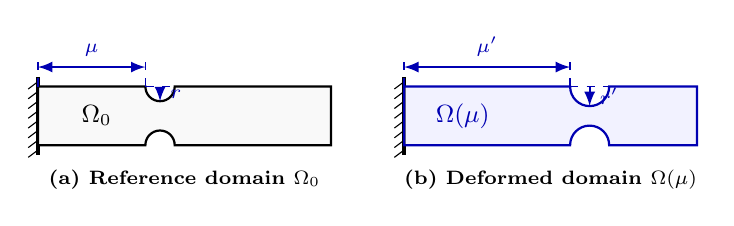
\begin{tikzpicture}[scale=0.62, >=stealth, every node/.style={font=\scriptsize}]
    \tikzset{
      reference/.style={thick, draw=black, fill=gray!5},
      deformed/.style={thick, draw=blue!70!black, fill=blue!10, fill opacity=0.5},
      dimension/.style={blue!70!black, <->, >=latex, line width=0.8pt},
      dimline/.style={blue!70!black, dashed, line width=0.5pt}
    }
    % --- PANEL 1: REFERENCE CONFIGURATION ---
    \begin{scope}[xshift=0cm]
      \draw[line width=1.5pt] (0,0.8) -- (0,-0.8);
      \foreach \y in {-0.7,-0.5,...,0.7} {\draw (0,\y) -- (-0.2,\y-0.15);}
      \draw[reference] (0,0.6) -- (2.2,0.6) arc (180:360:0.3) -- (6,0.6) -- (6,-0.6) -- (2.8,-0.6) arc (0:180:0.3) -- (0,-0.6) -- cycle;
      \node[black, font=\small] at (1.2, 0.0) {$\Omega_0$};
      \draw[dimline] (0, 0.6) -- (0, 1.1);
      \draw[dimline] (2.2, 0.6) -- (2.2, 1.1);
      \draw[dimension] (0, 1.0) -- (2.2, 1.0) node[midway, above] {$\mu$};
      \draw[dimline] (2.2, 0.6) -- (2.8, 0.6);
      \draw[blue!70!black, ->, >=latex, line width=0.8pt] (2.5, 0.6) -- (2.5, 0.3) node[midway, right] {$r$};
      \node[below, font=\scriptsize\bfseries] at (3.0, -0.9) {(a) Reference domain $\Omega_0$};
    \end{scope}
    
    % --- PANEL 2: PARAMETERIZED CONFIGURATION ---
    \begin{scope}[xshift=7.5cm]
      \draw[line width=1.5pt] (0,0.8) -- (0,-0.8);
      \foreach \y in {-0.7,-0.5,...,0.7} {\draw (0,\y) -- (-0.2,\y-0.15);}
      \draw[deformed] (0,0.6) -- (3.4,0.6) arc (180:360:0.4) -- (6,0.6) -- (6,-0.6) -- (4.2,-0.6) arc (0:180:0.4) -- (0,-0.6) -- cycle;
      \node[blue!70!black, font=\small] at (1.2, 0.0) {$\Omega(\boldsymbol{\mu})$};
      \draw[dimline] (0, 0.6) -- (0, 1.1);
      \draw[dimline] (3.4, 0.6) -- (3.4, 1.1);
      \draw[dimension] (0, 1.0) -- (3.4, 1.0) node[midway, above] {$\mu'$};
      \draw[dimline] (3.4, 0.6) -- (4.2, 0.6);
      \draw[blue!70!black, ->, >=latex, line width=0.8pt] (3.8, 0.6) -- (3.8, 0.2) node[midway, right] {$r'$};
      \node[below, font=\scriptsize\bfseries] at (3.0, -0.9) {(b) Deformed domain $\Omega(\boldsymbol{\mu})$};
    \end{scope}
  \end{tikzpicture}
  \vspace{0.1cm}
  
  \centering\small
  As $\boldsymbol{\mu}$ varies, the domain $\Omega(\boldsymbol{\mu})$ changes, causing \alert{vector space incompatibility}.
\end{frame}

% Slide: Governing Equations & Strong Form
\begin{frame}{Governing Equations \& Strong Form}
  \small
  Assuming small strains and a linear elastic isotropic material, the balance of linear momentum on $\Omega(\boldsymbol{\mu}) \times (0,T]$ is governed by:
  
  \begin{block}{Strong Form}
    \vspace{-0.1cm}
    \[
      \rho\,\ddot{\vect{u}} - \nabla \cdot \boldsymbol{\sigma}(\vect{u}) = \vect{f}_b \quad \text{in } \Omega(\boldsymbol{\mu}) \times (0,T]
    \]
  \end{block}
  \vspace{-0.1cm}
  with boundary and constitutive relations:
  \[
    \vect{u} = \vect{0} \text{ on } \Gamma_D(\boldsymbol{\mu}), \quad \boldsymbol{\sigma}(\vect{u})\cdot\vect{n} = \vect{h}_N \text{ on } \Gamma_N(\boldsymbol{\mu}), \quad \boldsymbol{\sigma}(\vect{u}) = \mat{D}:\boldsymbol{\varepsilon}(\vect{u})
  \]
  \vspace{-0.3cm}
  \[
    \boldsymbol{\varepsilon}(\vect{u}) = \tfrac{1}{2}\!\left(\nabla\vect{u} + (\nabla\vect{u})^T\right)
  \]
  \vspace{-0.2cm}
  \begin{itemize}
    \item $\rho$ — material density;\quad $\vect{f}_b$ — body force;\quad $\vect{n}$ — outward unit normal
    \item $\mat{D}$ — 4th-order elasticity tensor (reduces to $3\times3$ under plane stress)
  \end{itemize}
\end{frame}

% Slide: Pullback Mapping
\begin{frame}{Pullback Mapping to Reference Configuration}
  \small
  To enable shape ROM, equations on $\Omega(\boldsymbol{\mu})$ are mapped to a parameter-independent reference domain $\hat{\Omega}$ via a geometric diffeomorphism:
  \[
    \vect{x} = \boldsymbol{\Phi}(\hat{\vect{x}};\,\boldsymbol{\mu}), \quad \mat{J}(\hat{\vect{x}};\boldsymbol{\mu}) = \frac{\partial \boldsymbol{\Phi}}{\partial \hat{\vect{x}}}, \quad J_{\boldsymbol{\mu}} = \det\mat{J} > 0, \quad \mathrm{d}\Omega = J_{\boldsymbol{\mu}}\,\mathrm{d}\hat{\Omega}
  \]
  
  \begin{block}{Pulled-Back Weak Form on $\hat{\Omega}$}
    \vspace{-0.15cm}
    \[
      \hat{m}(\ddot{\vect{u}},\delta\vect{u};\boldsymbol{\mu}) + \hat{k}(\vect{u},\delta\vect{u};\boldsymbol{\mu}) = \hat{f}(\delta\vect{u};\boldsymbol{\mu}) \quad \forall\,\delta\vect{u}\in\mathcal{V}_0(\hat{\Omega})
    \]
    \[
      \text{where } \hat{k} = \int_{\hat{\Omega}} (\mat{J}^{-T}\nabla_{\hat{\vect{x}}}\vect{u}):\mat{D}:(\mat{J}^{-T}\nabla_{\hat{\vect{x}}}\delta\vect{u})\,J_{\boldsymbol{\mu}}\,\mathrm{d}\hat{\Omega}
    \]
  \end{block}
  \vspace{0.1cm}
  All parameter dependency is isolated into the Jacobian $\mat{J}(\hat{\vect{x}};\boldsymbol{\mu})$, keeping the mesh topology fixed.
\end{frame}

